\documentclass[
  a4paper,BCOR10mm,oneside,
  bibtotoc,idxtotoc,
  headsepline,footsepline,% also activate headinclude and footinclude
  fleqn,openbib
]{scrbook}
\usepackage[automark]{scrpage2}
\usepackage[ngerman,english]{babel}% default language as last entry
\usepackage[utf8]{inputenc}
\usepackage{amsmath} 
\usepackage{amsfonts}
\usepackage{amssymb}
\usepackage{graphicx}
\usepackage{lastpage}% to get last page use \pageref{LastPage}
\usepackage[refpage,intoc]{nomencl}% for nomenlature Abkuerzungsverzeichnis
\usepackage{listings}
\usepackage{color}
\usepackage{hyperref}
\usepackage{bm}
\usepackage{cleveref}
\usepackage{caption,setspace}
\definecolor{mygreen}{rgb}{0,0.6,0}
\definecolor{mygray}{rgb}{0.5,0.5,0.5}
\definecolor{mymauve}{rgb}{0.58,0,0.82}

\lstset{ %
  backgroundcolor=\color{white},   % choose the background color; you must add \usepackage{color} or \usepackage{xcolor}
  basicstyle=\footnotesize,        % the size of the fonts that are used for the code
  breakatwhitespace=false,         % sets if automatic breaks should only happen at whitespace
  breaklines=true,                 % sets automatic line breaking
  captionpos=b,                    % sets the caption-position to bottom
  commentstyle=\color{mygreen},    % comment style
  deletekeywords={...},            % if you want to delete keywords from the given language
  escapeinside={\%*}{*)},          % if you want to add LaTeX within your code
  extendedchars=true,              % lets you use non-ASCII characters; for 8-bits encodings only, does not work with UTF-8
  frame=single,	                   % adds a frame around the code
  keepspaces=true,                 % keeps spaces in text, useful for keeping indentation of code (possibly needs columns=flexible)
  keywordstyle=\color{blue},       % keyword style
  language=Octave,                 % the language of the code
  otherkeywords={*,...},           % if you want to add more keywords to the set
  numbers=left,                    % where to put the line-numbers; possible values are (none, left, right)
  numbersep=5pt,                   % how far the line-numbers are from the code
  numberstyle=\tiny\color{mygray}, % the style that is used for the line-numbers
  rulecolor=\color{black},         % if not set, the frame-color may be changed on line-breaks within not-black text (e.g. comments (green here))
  showspaces=false,                % show spaces everywhere adding particular underscores; it overrides 'showstringspaces'
  showstringspaces=false,          % underline spaces within strings only
  showtabs=false,                  % show tabs within strings adding particular underscores
  stepnumber=2,                    % the step between two line-numbers. If it's 1, each line will be numbered
  stringstyle=\color{mymauve},     % string literal style
  tabsize=2,	                   % sets default tabsize to 2 spaces
  title=\lstname                   % show the filename of files included with \lstinputlisting; also try caption instead of title
\makenomenclature
}

% define header and footer
\pagestyle{scrheadings}
\clearscrheadfoot % clear header and footer
\automark[section]{chapter}% !!! Wouldn't do that at oneside documents!!!
\ihead[]{\leftmark}% header left part
\ohead[]{\rightmark}% header right part
%\ifoot{Name}% footer left part
%\cfoot{Thema}% footer middle part
\makeatletter
% use different foot at front and main matter
\g@addto@macro{\mainmatter}{%
  \ofoot[{\usekomafont{pagenumber}Page \pagemark\ of \pageref{LastPage}}]
    {\usekomafont{pagenumber}Page \pagemark\ of 
      \pageref{LastPage}}% footer right part
}
\g@addto@macro{\frontmatter}{%
  \ofoot[\pagemark]{\pagemark}%
}
\makeatother


\begin{document}
\frontmatter% title pages are not numbered but counted!
\begin{titlepage}
  \raggedright% Use a different title style
  \null% page started
  \thispagestyle{empty}
  \selectlanguage{english}
  \vspace{4\baselineskip}
  \begin{tabular}{|ll@{}}
    & \\[\baselineskip]
    & \large Midtherm Report\\
    & \large Jan Grzegorzewski \\[\baselineskip]
    & \huge\textbf{Reaction-diffusion dynamics} \\
    & \huge\textbf{with fractional Brownian motion}\\[\baselineskip]
    & \large Summer term: 2016\\[2\baselineskip]
  \end{tabular}
\end{titlepage}

\tableofcontents
\listoffigures
%\listoftables

\mainmatter
\selectlanguage{ngerman}
\selectlanguage{english}
\printnomenclature
\clearpage

\newtheorem{mydef}{Definition}
\newcommand{\norm}[1]{\left\lVert#1\right\rVert}

\chapter{Introduction}
Anomalous diffusion can be observed in many different areas of nature, in particular related to heterogeneous media (Crowded biological media, porous materials, ...). The most popular phenomenon of anomalous diffusion is a power-law behaviour of the Mean-Square-Displacement ($MSD\propto t^{\alpha}$), which is violating the Einstein formula $MSD=2 d D t$ and thereby the central limit theorem. Various theoretical models try to encounter the power-law behaviour of the MSD showing different origins for anomalous diffusion. These models have the main phenomenon, thus the power-law behaviour of the mean square displacement, in common. But differ in some other observables, due to different origins of the anomalous power-law behaviour. By measuring theses different quantities one might reveal the origin of the anomalous behaviour in an experiment.\newline
One of these models which accounts this phenomenon is Fractional Brownian Motion. This thesis is going to focus on Fractional Brownian Motion especially in respect to Reaction and Diffusion Dynamics. (Normal Diffusion Limited Smoluchowski equation, chemical master equation, mass action law michaelis menden reaction ????? check it ) is failing miserably in describing Reaction and Diffusion Dynamics while anomalous motion is present.(explain ). The overall work aims not only to bring Reaction Diffusion and Fractional Brownian Motion together but also to provide a Fractional Brownian Motion Integrator implemented into a \textbf{Rea}ction \textbf{D}iffusion \textbf{Dy}namics software (ReaDDy). ReaDDy being a particle-based \textbf{Rea}ction \textbf{D}iffusion \textbf{Dy}namics software is acting on a macromolecular level. It is coarse-graining molecules into spherical particles. Usually using Brownian or Lagevin motion as the integrator. A Fractional Brownian Motion Integrator may be an elegant way of adding an approximation due to a crowded environment. The phenomenon of anomalous motion can also be studied with conventional integrators by actually building a crowded environment (for example: by adding obstacles). Nevertheless, the Fractional Brownian Motion approach could save computational time since it is not necessary to simulated each particle  explicitly which builds up the crowded environment. Furthermore different studies show that heterogeneous environments have influences on particle segregation in the presents of reactions.\newline
Having an Introduction set, chapter 2 deals with the theoretical foundation for Fractional Brownian Motion. Subsequently, due to computational reasons these theoretical elaborations need to be transferred into discrete space and finally casted into an algorithm. In the following some properties of the algorithm are studied. In Chapter 3, the theoretical foundation for reactions are going to be set. The final chapter 4 will deal with the present state of the thesis and give an outlook on further challenges.  

\chapter{Theory}
\section{Brownian Motion}
Fractional Brownian motion is a generalized case of standard Brownian Motion. The following section  will explore in more detail Brownian motion and normal diffusion. Than the more generalized case will be considerer. \newline
Standard Brownian Motion is a very important and good studied stochastic process. It describes the erratic motion for mesoscopic particles, which  first have been documented by Jan Ingenhousz in 1785, in particular for coal dust on the surface of alcohol. Later on in 1827 Robert Brown observed the erratic motion of pollen grains.  Brownian Motion has an Gaussian propagator which has its origin in the Central Limit Theorem (CLT) for a sum of of independent random variables. Lets assume a set of $N$ independent variables $\{X_i\}$ with a finite variance $ \sigma_i^2=\langle X_{i}^2\rangle $ and the mean $\langle X_{i}\rangle = 0$. The definition of a another random variable $Y$ is given by:
 \begin{align}
  Y = \frac{1}{\sqrt{N}} \sum_{j=1}^N X_j \label{eq:CLT}
 \end{align}
This scenario in which a random variable is defined of the sum of another can be observed generically in nature. In the following the distribution of Y, $\rho(y)dy=P(y<Y<y+dy)$ in the limit of large N, is going to be calculated. 
The Generating function for a random variable $Y$ is: 
\begin{align}
 G_Y(k)=\langle e^{ikY}\rangle = \int e^{ikY} \rho(y)dy
\end{align}
\cref{eq:CLT} can be inserted into the generating function, which results in:
\begin{align*}
G_Y(k)=\langle e^{\frac{ik}{\sqrt{N}} \sum_{j=1}^N X_j}\rangle \\
G_Y(k)=\langle \prod_{j=i}^N e^{\frac{ik}{\sqrt{N}} X_j} \rangle 
\end{align*}
If all $X_j$ are independent, then:
\begin{align}
 G_Y(k)= \prod_{j=i}^N \langle e^{\frac{ik}{\sqrt{N}} X_j} \rangle =e^{\sum_{j=1}^N A_j (\frac{k}{\sqrt{N}})} \\ \nonumber \text{ with } A_j(\frac{k}{\sqrt{N}})= ln \langle e^{\frac{ik}{\sqrt{N}} X_j} \rangle 
\end{align}
For large N behaviour, we assume $\frac{k}{\sqrt{N}} << 1$ and expand
\begin{align}
 A_j(\frac{k}{\sqrt{N}}) = ln(1+ \langle X_j \rangle \frac{ik}{\sqrt{N}} - \langle X_{j}^2 \rangle \frac{k^2}{2N}+\mathcal{O}(N^{- \frac{3}{2}}))
\end{align}
 with a finite variance $ \sigma_i^2=\langle X_{i}^2\rangle $ and the mean $\langle X_{i}\rangle = 0$
\begin{align}
 A_j(\frac{k}{\sqrt{N}}) = -\sigma_j^2 \frac{k^2}{2N}+\mathcal{O}(N^{- \frac{3}{2}}))
\end{align}

Thus, the generating function for large N is:

\begin{align}
 G_Y(k)=e^{- \frac{\sigma^2 k^2}{2}} \\ \nonumber
 \text{ with } \sigma =  \frac{1}{N} \sum_{j=1}^N \sigma_j^2 
\end{align}
The distribution of Y can be calculated via the inverse Fourier Transform:
\begin{align}
 \rho(y) &=\frac{1}{2 \pi} \int_{-\infty}^{\infty} e^{- \frac{\sigma^2 k^2}{2}} e^{i k y} dk \\  
 &=\frac{1}{\sqrt{2 \pi} \sigma } e^{-\frac{y^2}{2 \sigma^2}}
\end{align}
The seemingly innocent assumption of independence for the random variable $\{X_i\}$ in the summation results in an Gaussian distribution. Microscopic processes, which result in independent random position changes of an particle and add up over time, thus have a Gaussian distribution function for the overall position change. The propagator for Brownian motion has a Gaussian distribution.
\begin{mydef}
Standard Brownian motion is an stochastic process $ \{ W_t \}_{t\geq0}: \Omega \rightarrow \mathbb{R}^n$ with $ W_t(\omega)$ being the position of a particle with $\omega \in \Omega$ at time $t \in T$ in the observation time $T =[0, \infty)$. It has a fixed $x \in \mathbb{R}^n$ as its origin. The transition probabilities are: 
\begin{align}
T_{t}(y|x) & := (2 \pi t)^{- \frac{n}{2}} e^{- \frac{||x-y||^2}{2 t}} \text{for } y \in \mathbb{R}^n, t>0 \\ \nonumber
T_{0}(y|x) & = \delta(x-y) 
\end{align}
\end{mydef}
In the following some properties of Brownian motion are discussed:\\
\begin{itemize}
 \item Due to the Kolomogorov's continuity theorem a continuous path $ t \mapsto W_t(\omega)$ almost surely exists. Therefore it is possible to go to a continuous function $[0,\infty) \rightarrow \mathbb{R}^n$ and define a probability density.
\begin{align*}
p_{t_1,...,t_k}(x_1,...,x_k)  =T_{t_k -t_{k-1}}(x_k|x_{k-1}) ... T_{t_2 - t_1}(x_2|x_1) T_{t_1}(x_1|x)  \\
\text{ with }  0\leq t_1 < t_2 < ...< t_k,k \in \mathbb{N}
\end{align*}
\item Brownian motion is a Gaussian process with mean $E^x[W_t]=x$, $W_o=x$.
Since $ E^x[(W_{t_i}-W_{t_{i-1}})(W_{t_j}-W_{t_{j-1}})]=0 $  all its increments $\{W_{t_1},W_{t_2}-W_{t_1},...,W_{t_k}-W_{k-1}\}$ are independent.

\item Brownian motion has stationary increments since ${W_{t-h}-W_{h}}$ has the same distribution for all $h>0$.

\item Brownian scaling $\{\hat{W}_t := \frac{1}{c} W_{c^2 t} \}_{t\geq0}$ if $\{W_t\}_{t \geq 0}$  is also a Brownian motion. Therefore Brownian motion has self-similar and fractal paths.
\end{itemize}
For Brownian motion a linear relation between the MSD and the diffusion constant can be shown. The starting point is the diffusion equation for overdamped motion with a constant diffusion coefficient $D$. 
\begin{align}
 \frac{\partial}{\partial t} C(x,t) = - \frac{\partial }{\partial x} J (x,t) = D  \frac{\partial^2 }{\partial x^2} C(x,t) \label{eq:ficks}
\end{align}
Flux of particles  $J(x,t)=\frac{\partial }{\partial x} C(x,t)$ as a result of a linear response relation. 
Under this approximation diffusion only depends on the position and not on the velocity. Therefore it is again a long-time approximation for normal diffusion. The propagator of Brownian motion solves this equation. The Concentration $C(x,t)$ can be in interpreted as a probability distribution if properly normalized as $\int dx C(x,t)=1$. The Mean Square Displacement (MSD) can be calculated as:
\begin{align}
 \frac{d}{dt} \langle x^2(t)\rangle & =\frac{d}{dt} \int dx x^2 C(x,t)=\int dx x^2 \frac{\partial}{\partial t} C(x,t) \\
&= D \int_{-\infty}^{\infty}dx x^2 \frac{\partial^2 }{\partial x^2} C(x,t) = -2 D \int_{-\infty}^{\infty} dx x \frac{\partial }{\partial x} C(x,t) \\ &= 2 D \int_{-\infty}^{\infty} dx C(x,t) =2 D
\end{align}
In previous equations partial integration has been used and  $C(\pm \infty,t)=0$ has been assumed. By integration, for the initial condition $x(0) = 0$,  one gets the Einstein Formula: $\langle (x(t)-x(o))^2)\rangle= 2Dt$, which can easily be extended for 2 and 3 dimensions. It will not be calculated here explicitly, but one can show that also for the  Smoluchowski eq. which follows from langevin dynamics for a long time limit the initial velocities decorrelate and thus the MSD is also linear with time.

\section{Fractional Brownian Motion}
In this section the theoretical foundation for Fractional Brownian Motion will be set and related to standard Brownian Motion. \\
In the previous section the the Means Square Displacement (MSD) has been shown to be linear with time as a result of the central limit theorem. In normal liquids this behaviour can be be seen already at time scales higher than picosecends \cite{Hofling2013}. Nevertheless many experiments show that the MSD has a power law behaviour ( $\delta r ^2 (t) \propto t^{\alpha}$ for  $0 < \alpha < 1$ ). Thus the central limit theorem does not hold, not even for long time scales. It can be shown that persistent correlations of the increments are present. In soft matter, like polymers, subdiffusive behaviour is typically present in an time window but finally the linear MSD takes over. Fractional Brownian Motion instead examines the case that the central limit theorem is violated for all time scales.\\
In the following some statistical tools are defined. They are important as the increments of Fractional Brownian motion are no longer assumed to be independent. The single particle density $\rho(\bm{r},t)=\delta(\bm{r}-\bm{R}(t))$ describes the density of a particle which is localized at position $\bm{R}(t)$. Its correlation function $P(\bm{r}-\bm{r}',t-t')= V\langle\rho(\bm{r},t) \rho(\bm{r}',t')\rangle$ is also called Van Hove self-correlation function. $V$ refers to the volume. From now on we will consider an isotropic system $ r= |\bm{r}|$. As for Brownian motion with independent increments the correlated increments  $\Delta\bm{R}(t)$ of fractional Brownian motion are assumed to follow a Gaussian distribution with zero mean. Thus the correlation function of the single particle density results in:
\begin{align}
 P(r,t)=[2 \pi \delta r^{2}(t)/d]^{-\frac{d}{2}} e^{ \frac{-r^2 d}{2 \delta r^{2}(t) }}
\end{align}
The van hove correlation function can be transformed via the spatial Fourier transform into the wave-number representation, which is called the self-intermediate scattering function. Again for isotropic systems one can write $|\bm{k}|=k$.
\begin{align}
 F_{s}(k,t)&=\langle\rho(k,t) \rho(k',t')\rangle=\int d^{d}r e^{-i k r} P(r,t) \\
 &=\langle e^{-i k \Delta R(t)} \rangle
\end{align}
The intermediate scattering function for the single particle density turns out to be the characteristic or moment generating function of $\Delta R(t)$ by expanding it for small wave-numbers $k \rightarrow 0$ one can get the moments. Its logarithm return the cumulants. For Gaussian propagators all but the second cumulants vanish. For non Gaussian transport also the fourth cumulant is non-zero. Therefore it is used to indicate beyond Gaussian transport.The non-Gaussian parameter is defined as:
\begin{align}
 \alpha_2=\frac{d \delta r^{4}(t)}{(d+2) [\delta r^{2}(t)]-1}
\end{align}
An other important quantity is the dynamical structure factor, which is the time-frequency Fourier transform of the intermediate scattering function:
\begin{align}
 F_{s}(k,z)&=\langle\rho(k,z) \rho(k',z')\rangle=\int_{0}^{\infty} d t e^{-i k r} P(r,t) \text{ for } k \rightarrow 0 , \operatorname{Im}(z) > 0 \\
 &= \frac{1}{-iz}-\frac{k^2}{2d}\int_{0}^{\infty} d t e^{izt} \delta r^2 (t) + \mathcal{O}(k^2)
\end{align}
From now on lets start from a differential equation $\partial_t \bm{R}(t)=\bm{\eta}(t)$. $\bm{\eta}(t)$ are velocities, which are no more delta-correlated in time as they would be for standard Brownian motion. Velocities can be used to calculated the Velocity Autocorrelation Function (VACF):
\begin{align}
Z(|t-t'|)&= \frac{1}{d}\langle \bm{\eta}(t) \bm{\eta}(t') \rangle = \frac{1}{2d} \frac{d^2}{dt^2} \delta r^2 (t-t')  \\
\end{align}
Subsequently, the VACF in the frequency domain for Fractional Brownian motion can be calculated. The MSD is $\delta r^{2}(t)= < \Delta R(t)>=2dK_{\alpha}t^{\alpha}$ with $K_{\alpha}$ being the generalized diffusion-coefficient:
\begin{align*}
 \tilde{Z}(z)&=\int_{0}^{\infty} d t e^{izt} Z(t) \\
 &=2 d \int_{0}^{\infty} d t e^{izt} \left[\frac{d^2}{dt^2}\delta r^2 (t) \right]
\end{align*}
\begin{align*}
  \stackrel{par. integ.}{=} 2d \left( \underbrace{\left [ e^{izt}\overbrace{ \frac{d^2}{dt^2} 2dK_{\alpha}t^{\alpha}}^{=A(t)} \right]_{0}^{\infty}}_{\stackrel{\alpha < 2} {=} 0}-\int_{0}^{\infty} d t e^{izt} \left[\frac{d}{dt}\delta r^2 (t)\right] \right) 
 \end{align*}
 \begin{align*}
 A(t)=\frac{d}{dt}\overbrace{ \left [\frac{2d K_{\alpha}t^{\alpha-1}}{\alpha} \right ]}^{B(t)}=\frac{2d K_{\alpha}t^{\alpha-2}}{\alpha+(\alpha-1)}
\end{align*}

\begin{align*}
 \tilde{Z}(z) & \stackrel{par. integ.}{=} - 2d \left( \underbrace{\left [ e^{izt}\overbrace{ \frac{d}{dt} 2dK_{\alpha}t^{\alpha}}^{=B(t)} \right]_{0}^{\infty}}_{\stackrel{\alpha < 1} {=} 0}-\int_{0}^{\infty} d t e^{izt} \delta r^2 (t) \right) \\
  & = \int_{0}^{\infty} d t e^{izt} \delta r^2 (t)  \stackrel{\operatorname{Im}(z)> 0} {=}  K_{\alpha} \Gamma(1+\alpha)(i z)^{1-\alpha}
\end{align*}
Eventually, the VACF in the frequency domain will be used to modify standard Brownian motion velocities, which are easily computable, to generate fractional Brownian motion velocities. The  starting point is again the differential equation $\partial_t \bm{R}(t)=\bm{\eta}(t)$. In the frequency domain they are represented as:
\begin{align}
 \tilde{\bm{\eta}}(z)=\int_{0}^{\infty} dt e^{izt} \bm{\eta}(t) \label{eq:fourier}
\end{align}
Fractional correlations can be incorporated via its VACF:
\begin{align}
\tilde{\bm{\xi}}(z) = \sqrt{2 \operatorname{Re} \left(\tilde{Z(z)}\right)}  \tilde{\bm{\eta}}(z) \label{eq:fracvacf}
\end{align}
 With $\tilde{\bm{\xi}}(z)$ being fractional Brownian velocities in the frequency domain. Its Fourier-back-transform results in Fractional Brownian velocities in the time domain.
 \begin{align}
 \bm{\xi}(t)= \frac{1}{2 \pi} \int dz\tilde{\bm{\xi}}(z)
 \end{align}

\subsection{Algorithm}
In the following an algorithm which generates fractional Brownian noise will be introduced. The algorithm is based on the Davis-Harte algorythm \cite{Craigmile2003}. The idea is to use the calculated VACF and thereby modify conventionally generated Gaussian random variables.  All the increments should be generated beforehand. With this concept it is more difficult to include forces. Nevertheless it is computationally favourable then computing each increment recursively considering also its history. This would be certainly necessary since all increments are defined to be more then just delta-correlated in time. For computational reasons the elaborations for fractional Brownian motion in the previous chapter on how to generate fractional Brownian increments have to be transformed into a discrete form, thereby the solution is no longer exact, which will be shown in the analyse part of the algorithm.   
\begin{align}
\bm{\eta} (t) \longrightarrow \bm{\eta}_j(t)  \text{  with  } j=0,1,2,...,n  \text{  ,  } n= \text{amount of steps}
\end{align}
For a n-steps long trajectory one can write:
\begin{align}
 \Delta \bm{R}_n(t) =  \sum_{j=0}^n \bm{\eta}_j  \Delta t \label{eq:diskretdeltar}
\end{align}

 The following algorithm is explained for one dimension and can be easily extended for more dimensions. The MSD then can be written as:
\begin{align}
< \Delta R_{j}(t)>=2K_{\alpha} (\Delta t j)^{\alpha}
\end{align}
The algorithm goes as follows:
\begin{enumerate}
 \item $2 n$ independent normally distributed random increments are generated: 
\begin{align}
 \eta_k(t)= \mathcal{N}(0,\sqrt{\Delta t}) \text{  with  } k=0,1,2,...,2n
\end{align}

$2$ times more increments are generated to counteract the boundary problem in the discrete Fourier transform. 

\item Via discrete Fourier transform these increments are transformed into the frequency domain:
\begin{align}
 \tilde{\eta_l}(z)=\sum_{k=0}^{2n-1} \eta_k e^{\frac{- i 2 \pi  l k }{2n}} \Delta t   \text{  with  }  l=0,1,2,...,2n  \label{eq:fouriertrans}\\ 
\end{align}
By comparison with the \cref{eq:fourier} one can see that:
\begin{align}
 z \rightarrow  l \Delta z \text{ , } \Delta z =   \frac{2 \pi }{2n \Delta t} \text{ , } t \rightarrow j \Delta t \text{ and } \int dt \rightarrow \sum \Delta t \label{eq:diskret-freq} 
\end{align}
 
\item Comparable to \cref{eq:fracvacf} correlations are incorporated: 
 \begin{align}
   \tilde{\xi}_{l}(z)&= \tilde{\eta}_l(z) \sqrt{2 Re( \tilde{Z}_l(z))} \label{eq:corelastion} 
  \end{align}
 with $\tilde{Z}(z)\rightarrow \tilde{Z}_l(z)$ as introduced in \cref{eq:diskret-freq}:
  \begin{align}
   \tilde{Z}_l(z) = K_{\alpha} \Gamma(1+\alpha)(i 2 \pi l \Delta z)^{1-\alpha} =  K_{\alpha} \Gamma(1+\alpha)(i l \frac{ \pi}{n \Delta t})^{1-\alpha} 
 \end{align}
 
 \item The discrete Fourier transform has a downside compared to the continuous Fourier transform, as already noted in the beginning of this section. The VACF is zero at zero-frequency $ \tilde{Z}_{l=0}(z=0)=0$.  From \cref{eq:corelastion} also the first increment in the frequency domain is zero $ \tilde{\xi}_{l=o}(z=0)= 0$. Due to \cref{eq:fouriertrans} also the following relation holds:
 \begin{align}
   \tilde{\xi}_{l=o}(z) = \sum_{k=0}^{2n-1} \xi_k e^{0} \Delta t = \Delta  R_{2n}
 \end{align}
$\Delta R $ is the distance between the starting point and the position of the particle. Therefore the particle would travel after $2n$ steps back to its initial position. Instead the zero-increment in the frequency domain is calculated as follows:
\begin{align}
 \tilde{\xi}_{l=o}(z) = \mathcal{N}(0,\sqrt{2 K_{\alpha} (2n \Delta t)^\alpha})
\end{align}
 This equation would be correct if we assumed fractional Brownian motion to be a Markovian process which certainly is not the cause. This is also the reason why k have been chosen to be $2n$. The presumption is, that the impact of the approximation would be negligible with increasing distance to $\Delta R_{2n}$ and negligible at $\Delta R_{n}$.  
 %\item Laut dem Davies Harte Algorithmus wird außerdem das n-te Inkrement im Frequenzraum %umgeändert:
 %\begin{align}
 %\eta_{fbr_{g=n}} =\sqrt{Re(Z_g 2 n)} \mathcal{N}(0,1) 
 %\end{align}
 % Noch nicht verstanden warum!!
 \item With the reverse Fourier transform the fractional Brownian noise increments in the time domain result in:
 \begin{align}
 \xi_{k}= \frac{1}{2n} \sum_{l=0}^{2n-1}  \tilde{\xi}_l e^{\frac{2 \pi i l k }{2n}} \Delta z
 \end{align}
Only the first half of the increments are taken  into account $\xi_{j}$ für $j=(0,1,..,n)$.
\end{enumerate}
The described algorithm can be performed for every Cartesian component of the three dimensional fractional Brownian motion. The Cartesian component are not correlated.
\subsubsection{Analyse of Algorythm}

\begin{figure}[h]
\centering
\begin{minipage}{.5\textwidth}
  \centering
  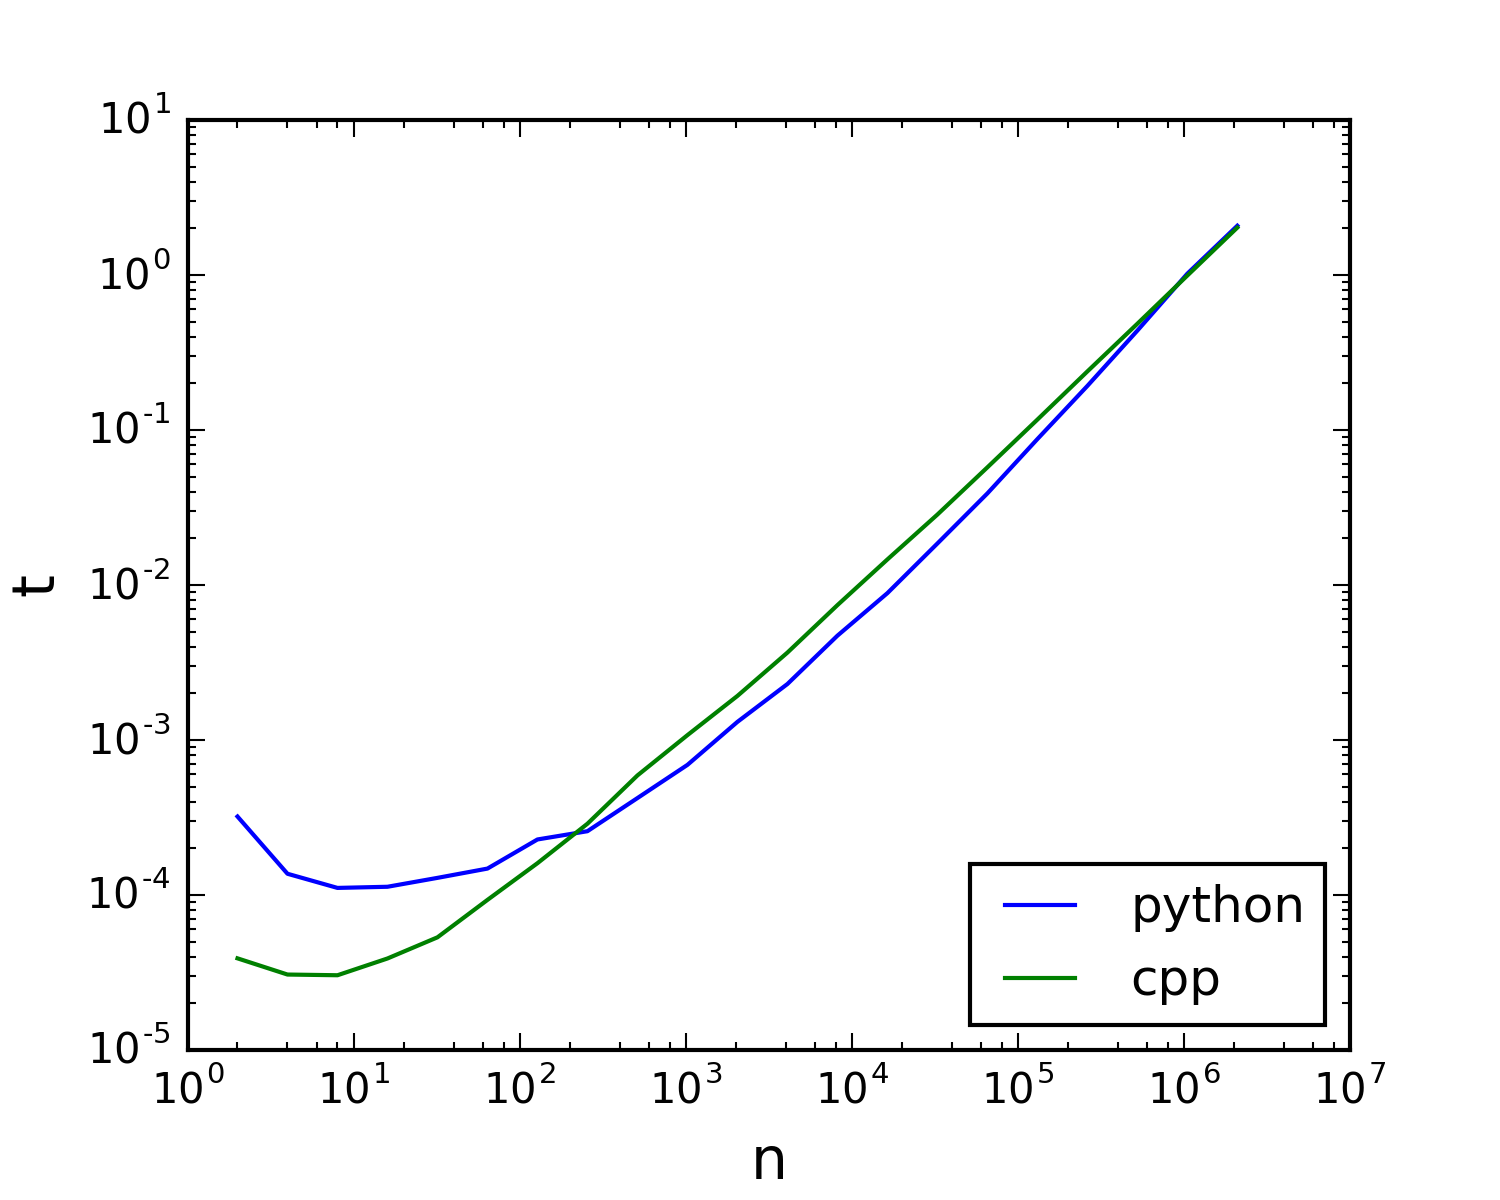
\includegraphics[width=\linewidth]{./data/profiling_length.png}
  \captionsetup{width=0.9\linewidth}
  \captionof{figure}{Profiling c++ and python code in respect to trajectory length $n$}
  \label{fig:test1}
\end{minipage}%
\begin{minipage}{.5\textwidth}
  \centering
  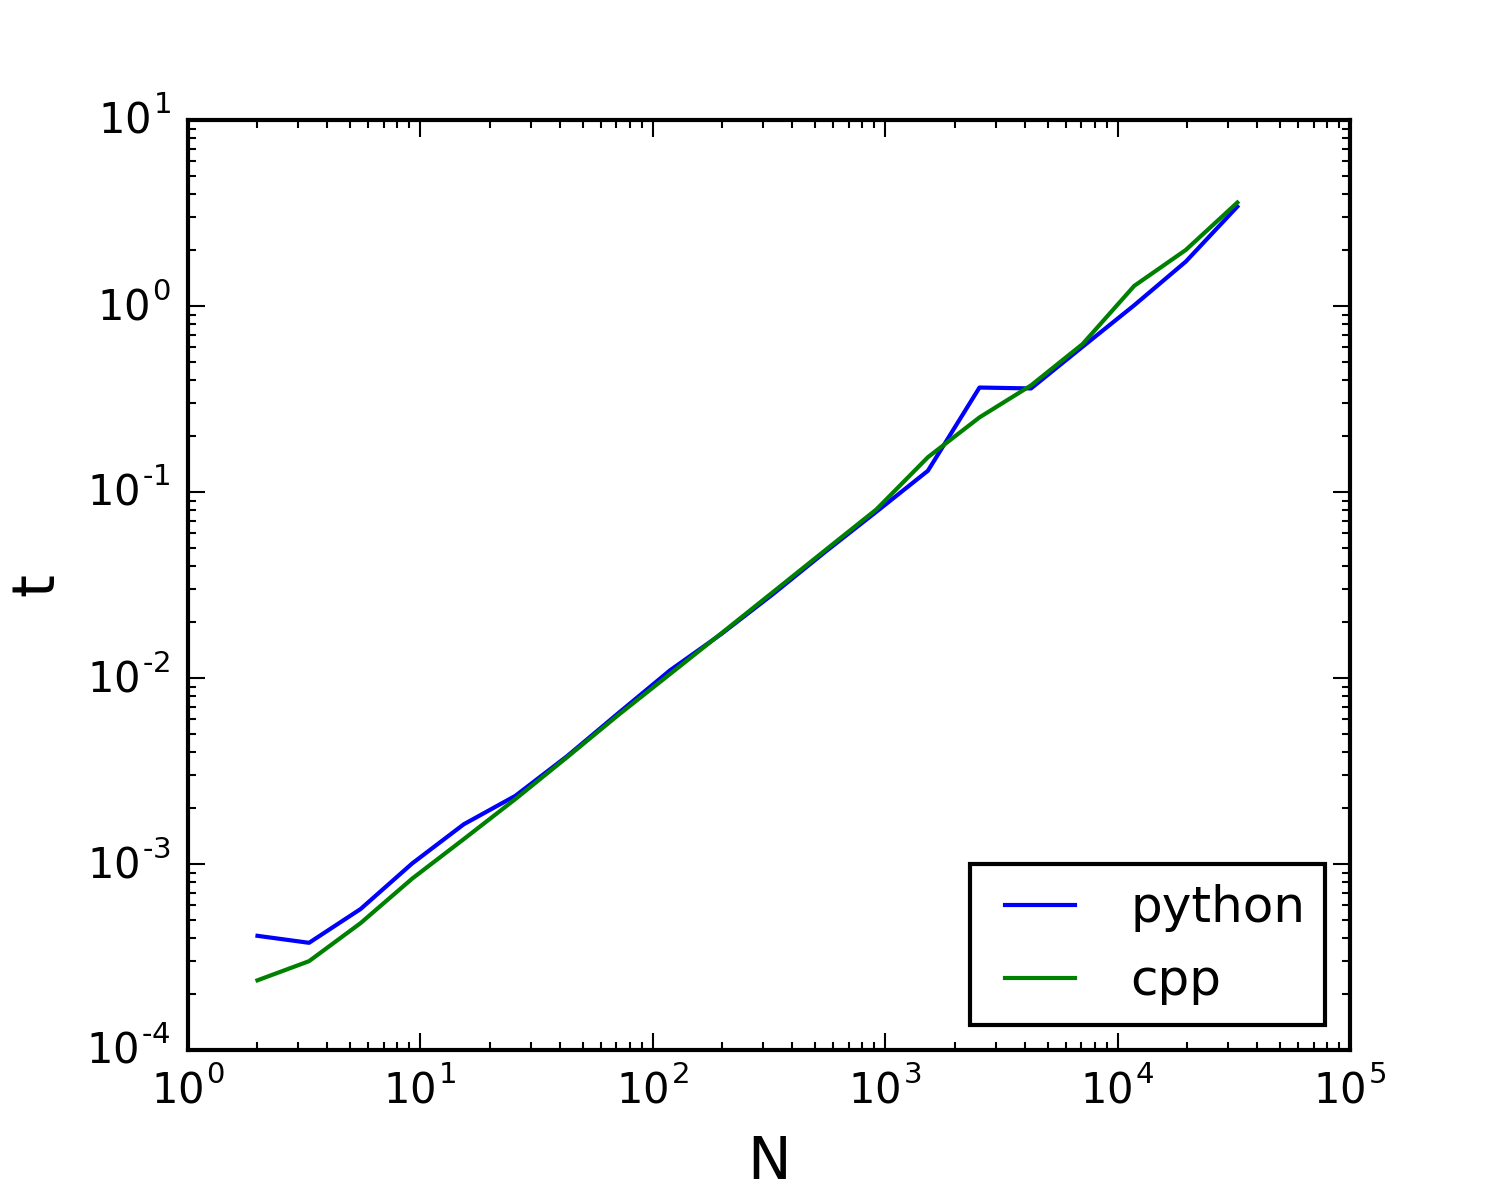
\includegraphics[width=\linewidth]{./data/profiling_particle.png}
  \captionsetup{width=0.9\linewidth}
  \captionof{figure}{Profiling c++ and python code in respect to trajectory number $N$}
  \label{fig:test2}
\end{minipage}
\end{figure}

\begin{figure}[h]
\centering
\begin{minipage}{.5\textwidth}
  \centering
  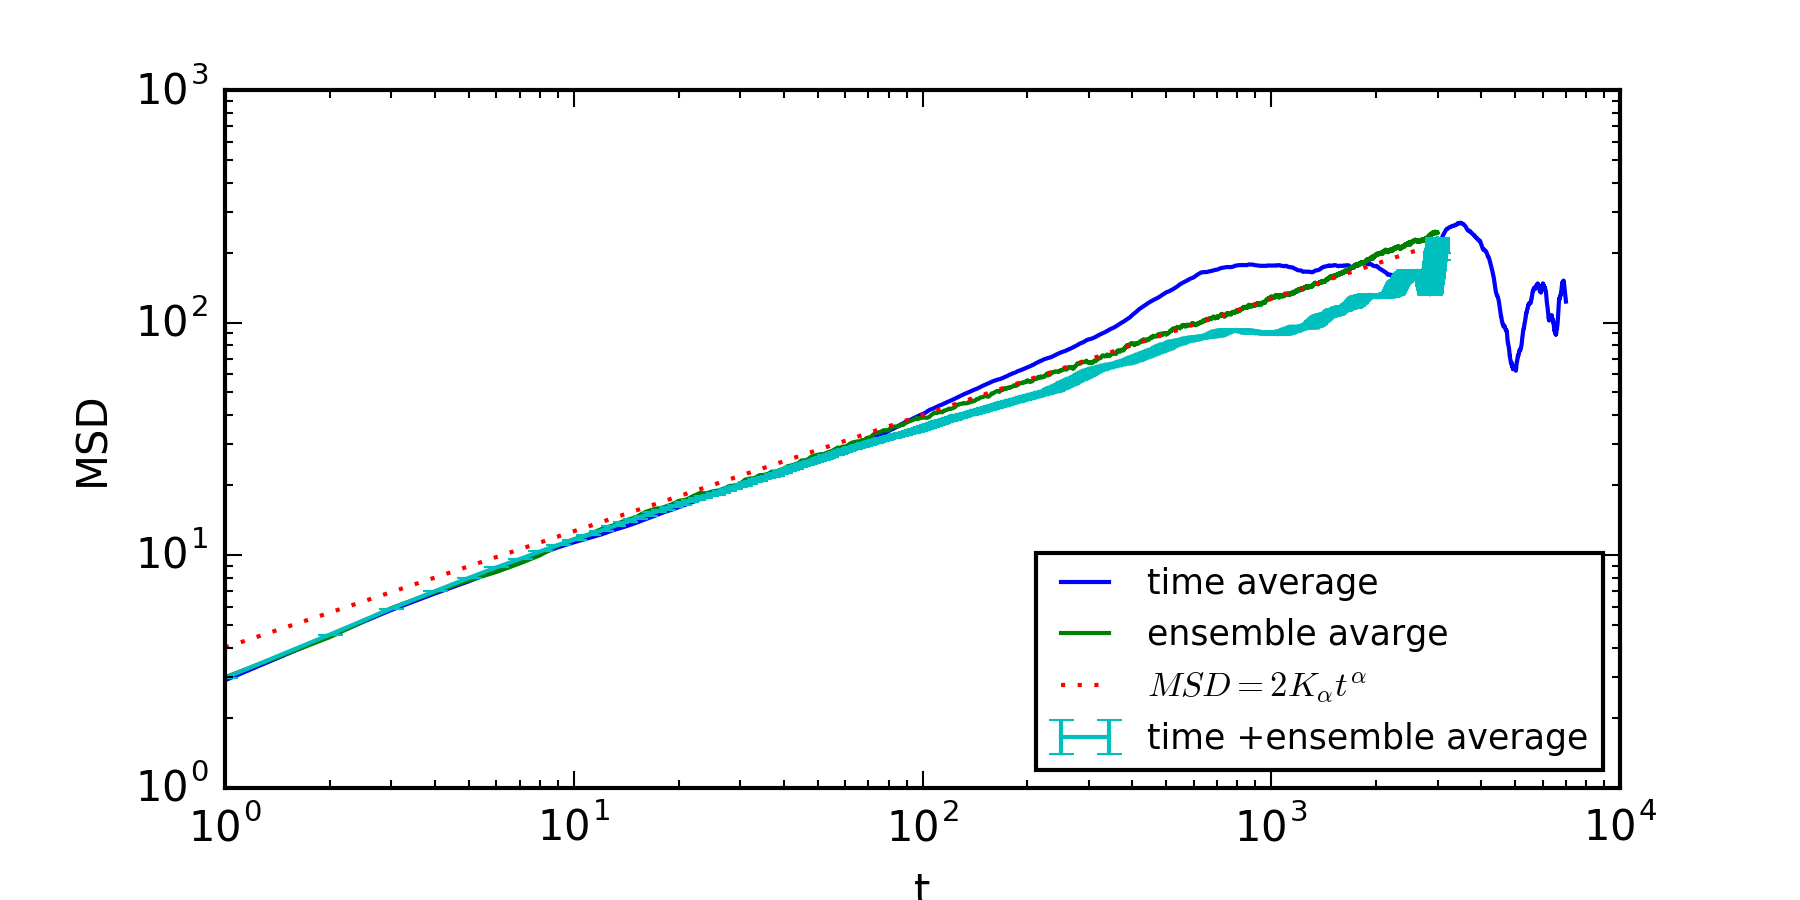
\includegraphics[width=\linewidth]{./data/averages_comparison.png}
  \captionsetup{width=0.9\linewidth}
  \captionof{figure}{Comparison of Mean-Square-Displacements between time-average, ensemble-average and time-ensemble-average(for $D=2$, $\alpha=0.5$, $\Delta t=1$). }
  \label{fig:test1}
\end{minipage}%
\begin{minipage}{.5\textwidth}
  \centering
  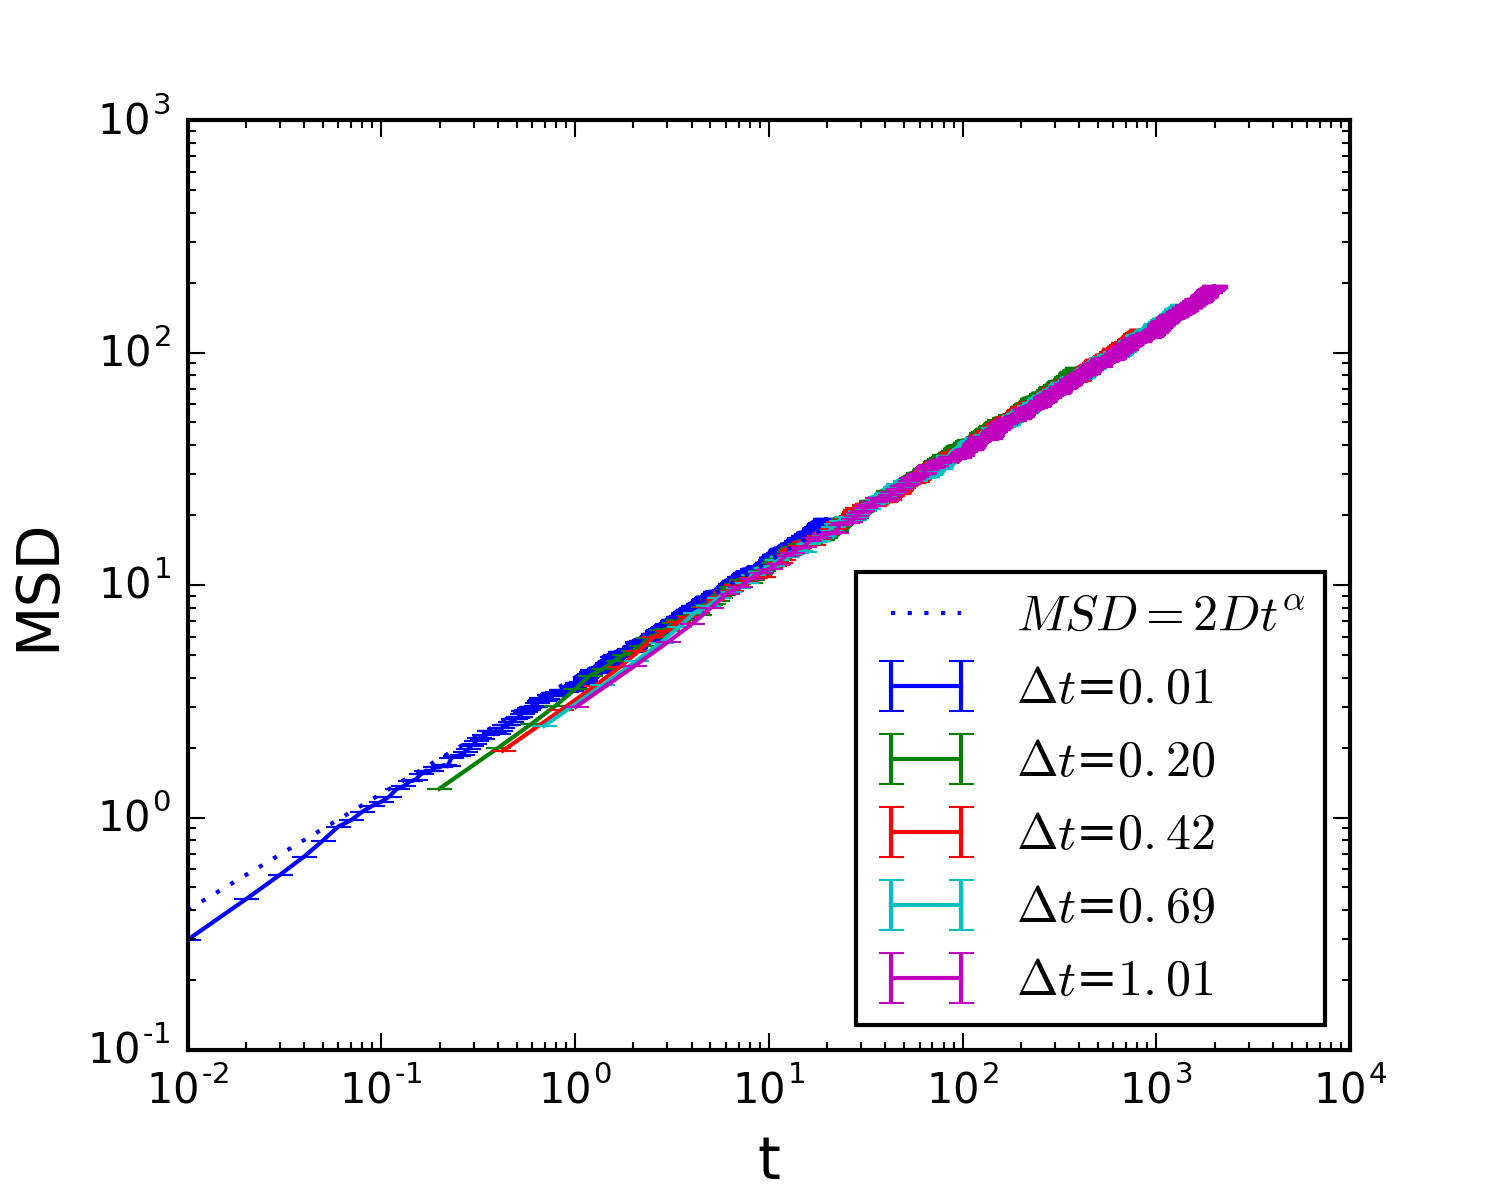
\includegraphics[width=\linewidth]{./data/dt_change.png}
  \captionsetup{width=0.9\linewidth}
  \captionof{figure}{Comparison of ensemble averaged Mean-Square-Displacements with different $\Delta t$(for $D=2$, $\alpha=0.5$). }
  \label{fig:test2}
\end{minipage}
\end{figure}


\begin{figure}[h]
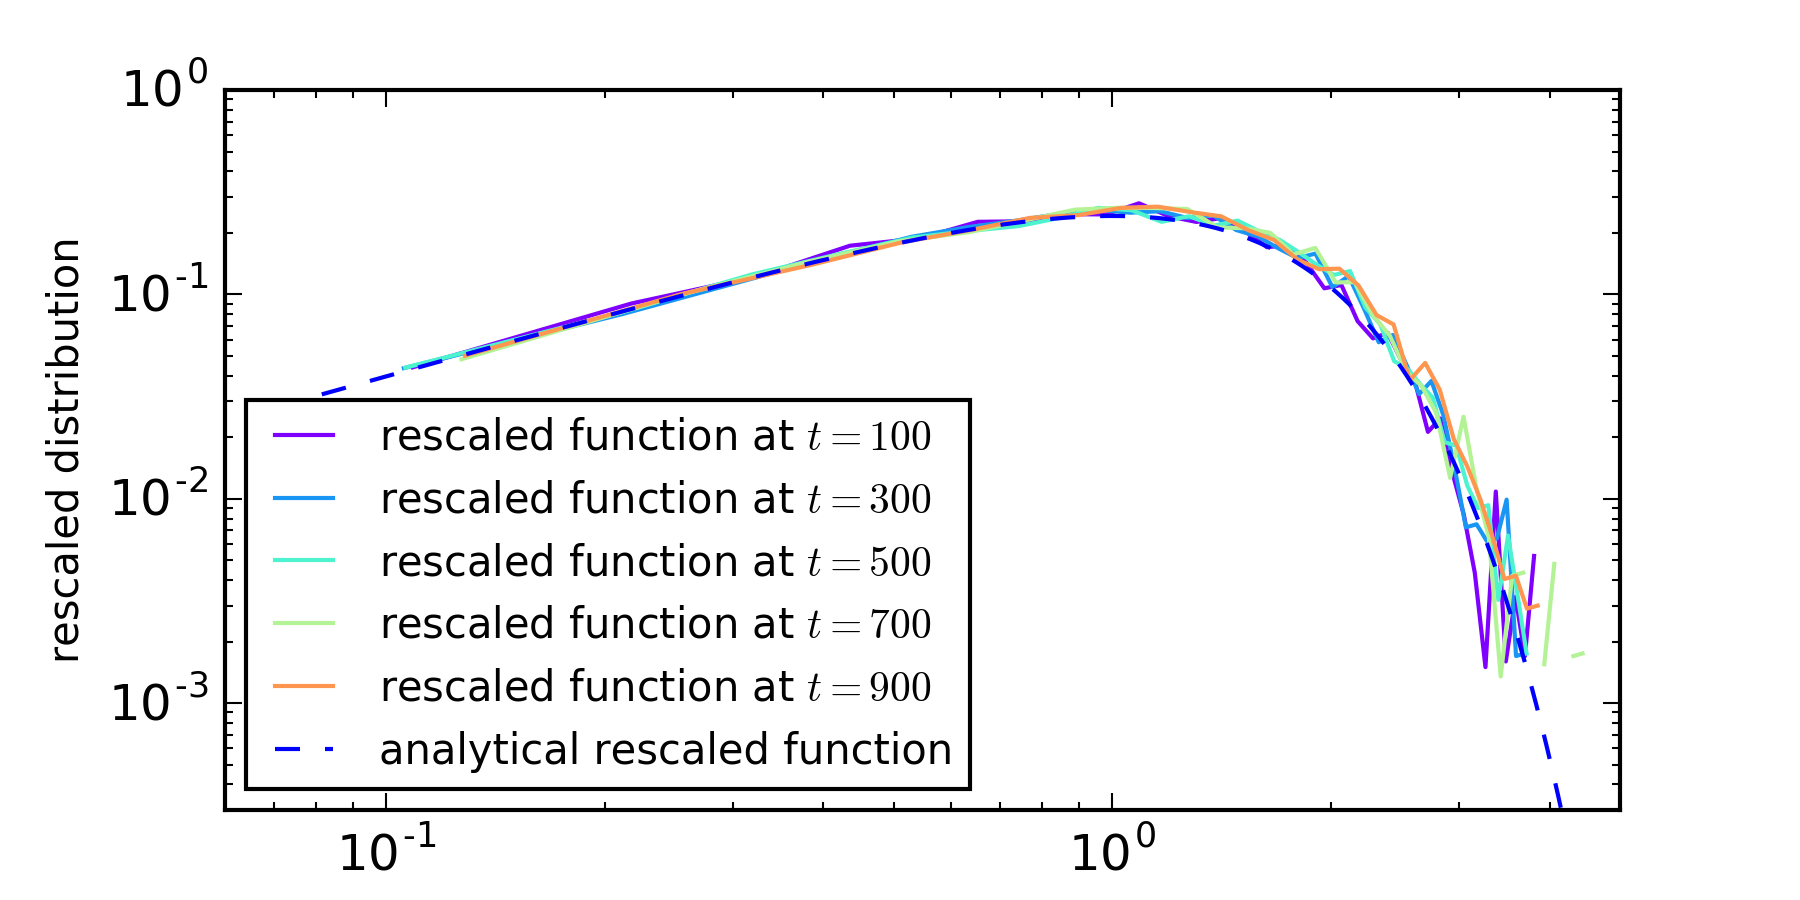
\includegraphics[width=\textwidth]{./data/rescaled.png}
\caption{rescaled functions}
 \centering
\end{figure}

\begin{figure}[h]
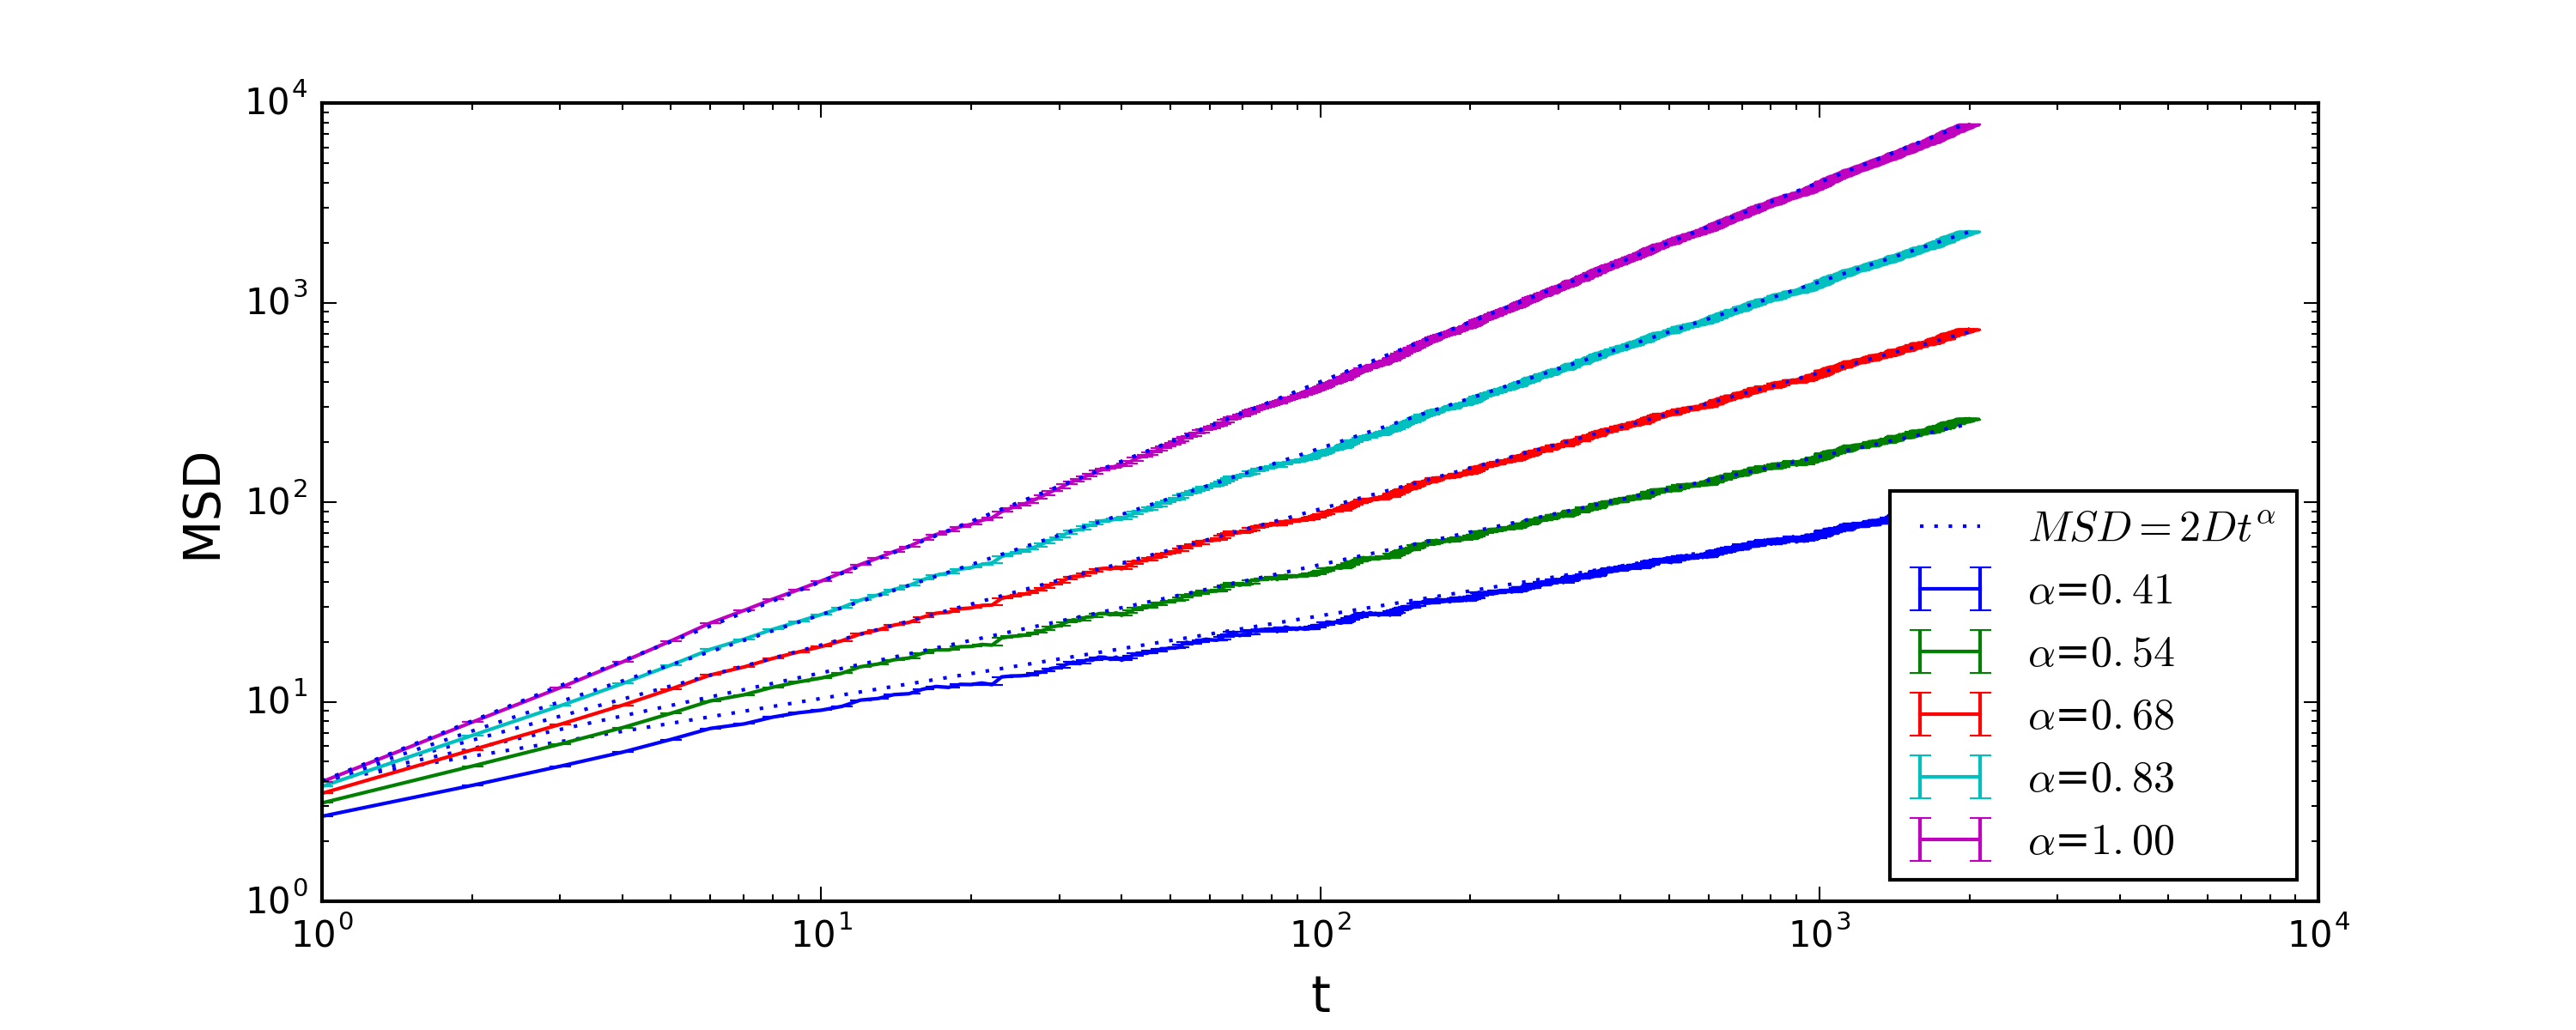
\includegraphics[width=\textwidth]{./data/alpha_change.png}
\caption{Mean-Square-Displacement for different $\alpha$. With $K_{\alpha}=2$ , $N=2000$, $n=2000$ , $\delta t = 1$, $M=2n$ }
 \centering
\end{figure}

\begin{figure}[h]
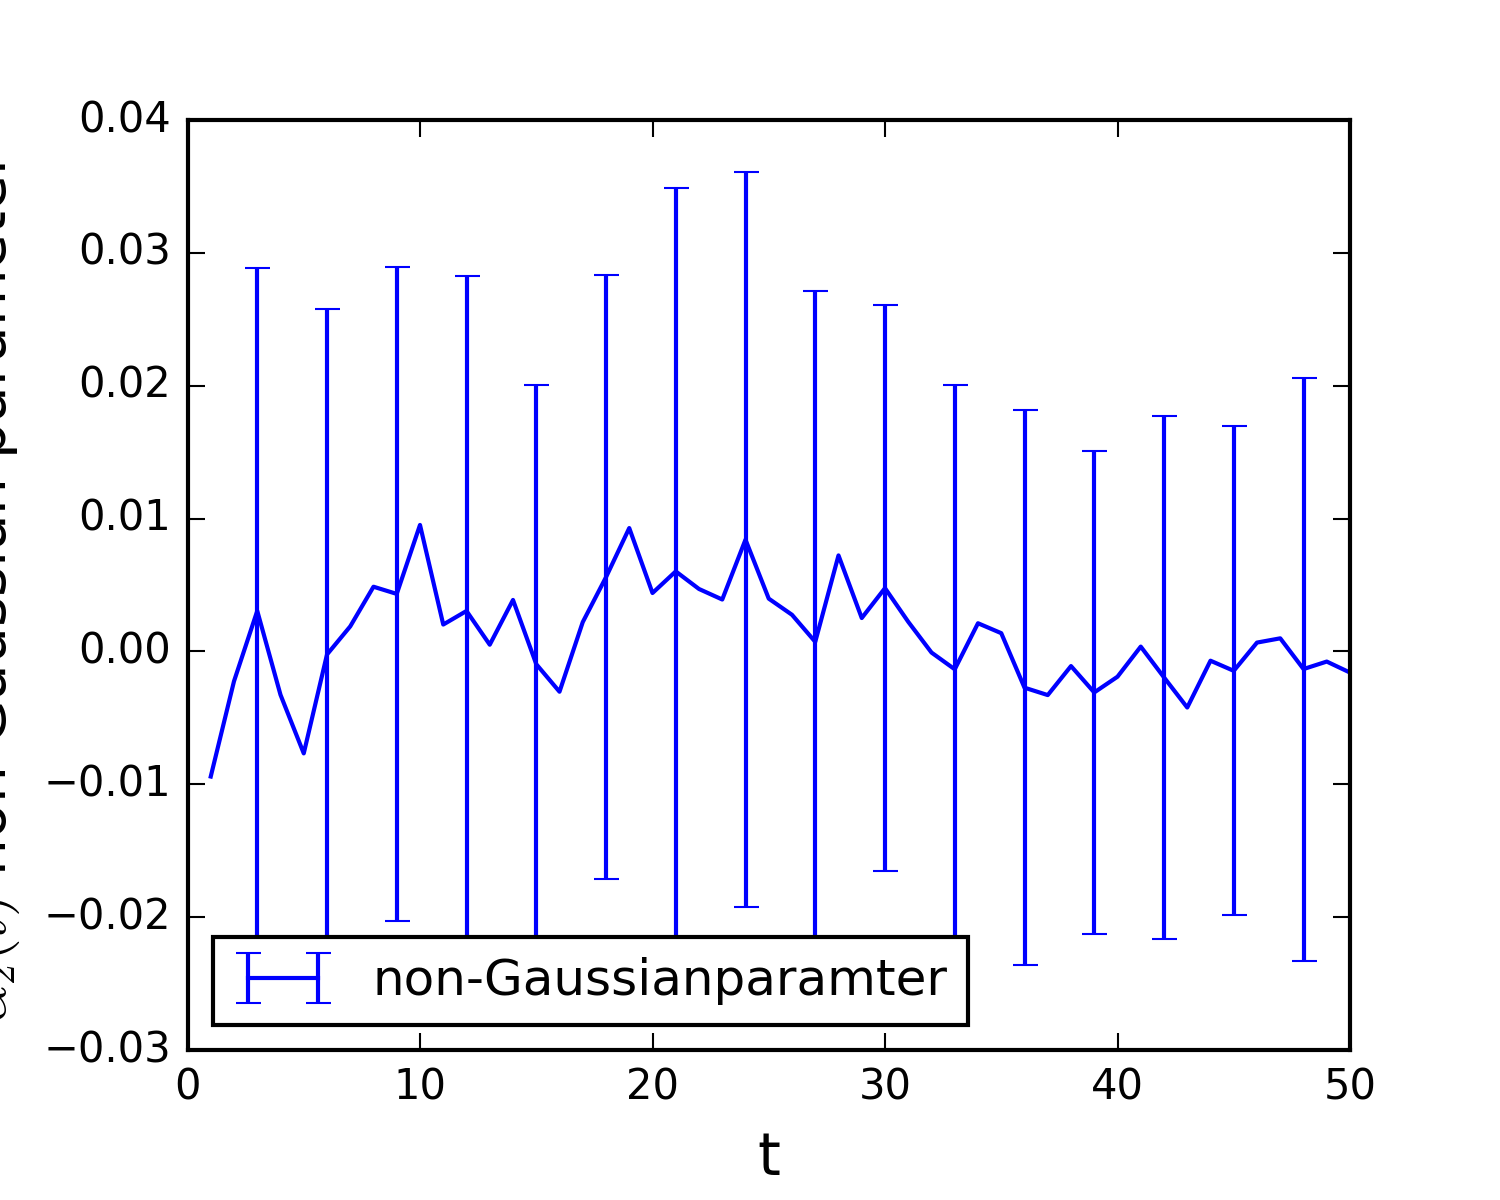
\includegraphics[width=\textwidth]{./data/nongaussian.png}
\caption{Non-Gaussian-Parameter With $K_{\alpha}=2$ , $N=5000$, $n=1001$ , $\delta t = 1$, $M=2n$ averaged over $30$ non-Gaussian-Parameter}
 \centering
\end{figure}




\chapter{Reactions-Diffusion-Dynamics}
\chapter{Status Quo \& Outlook}
%\chapter{Appendix}
%\subsection{Code:Gebrochen-rationale Brownische Bewegung}
%\lstinputlisting[language=Python]{../simulation.py}

\nocite{}

%\printindex
\bibliography{literatur}
\bibliographystyle{plain}
\url{http://wwo.weizmann.ac.il/weizsites/mukamel/files/2013/01/Brownian_Motion.pdf}

\end{document}